\section{Neutrinos, Backgrounds, and Routing}

A valid full reconstruction requires all packets to be collected regardless of neutrino type, energy within the valid range, interaction vertex, and should also be able to accept a range of incoming momentum angles.
In this final section of the chapter we combine the results of the neutrino interactions as well as the radiogenic and leakage backgrounds into the simulation framework described in Section~\ref{sec:tile_simulation}, which is based on the graph developed in Chapter~\ref{chap:qdb}.
This back-end simulation framework is also my sole and independent work.

\subsection{Combining the Digital and Physical Simulations}

To synthesize the results of the neutrino events and the background sources we take a reference 10 second window slice from a 1000 second simulation of backgrounds as described in Section~\ref{sec:simulating_tile}.
We then select a single $\nu_{e}$ interaction from the forward horn current direction, where we accept any incoming $\theta_{z}$, z-position, and energy.
This event is offset to occur at time: $\tau_{int} = $5.1 seconds.
We do not perform this readout simulations for all parameters in Table~\ref{table:neutrino_params} as Figure~\ref{fig:compare_integral_pdg} indicates that the local buffer requirement does not largely depend on neutrino flavor.

We choose $\tau_{int} = 5.1~\unit{s}$ so that the interaction occurs just after interrogation request from the aggregator node.
This ensures that the entire $\nu_{e}$ interaction is buffered onto all local FIFOs in the tile before the request. 
We note that this time offset is the same for the push architecture, even though the neutrino reset packets will be sent when they are acquired.

\subsection{Remote FIFO Depth Results}

Figure~\ref{fig:mp60_slow_plots_for_digital_sim} shows combined results for the remote transactions, remote FIFO depth, and 99\% capture requirements.
The remote transactions for both the left and trunk routings are much smaller on average than the snake routing for the reasons described in Section~\ref{sec:simulating_tile}.

The Table~\ref{tab:transact} contains the results for the effect the different routings have on the average number of transactions.

The Table~\ref{tab:buffers} summarizes the results of Plot-(B) in Figure~\ref{fig:mp60_slow_plots_for_digital_sim} for the parameters described in Table~\ref{table:tile_params}.

The Table~\ref{tab:fit} summarizes the linear fit results of Plot-(D) in Figure~\ref{fig:mp60_slow_plots_for_digital_sim} for the parameters described in Table~\ref{table:tile_params}.
The final column of this table indicates the relative fit from the push-based architecture, for which only the snake routing was tested.

%%% Example of Digital Simulation Reconstruction
\begin{figure*}
  \centering
  \begin{subfigure}[b]{0.475\textwidth}
      \centering
      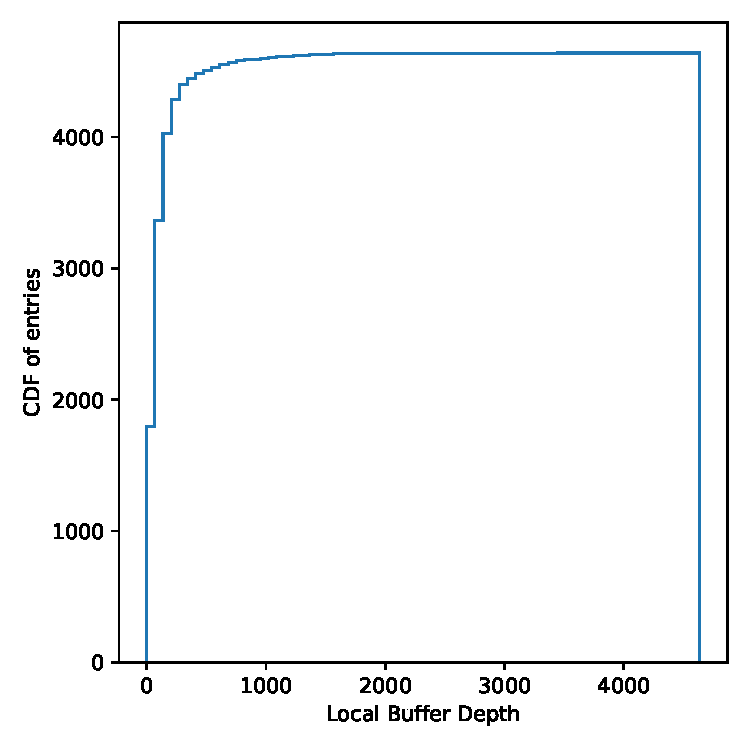
\includegraphics[width=\textwidth]{./images/mp60_16_slow_local_stack.pdf}
      \caption[]%
      {{\small Local Buffer Capture}}    
  \end{subfigure}
  \hfill
  \begin{subfigure}[b]{0.475\textwidth}  
      \centering 
      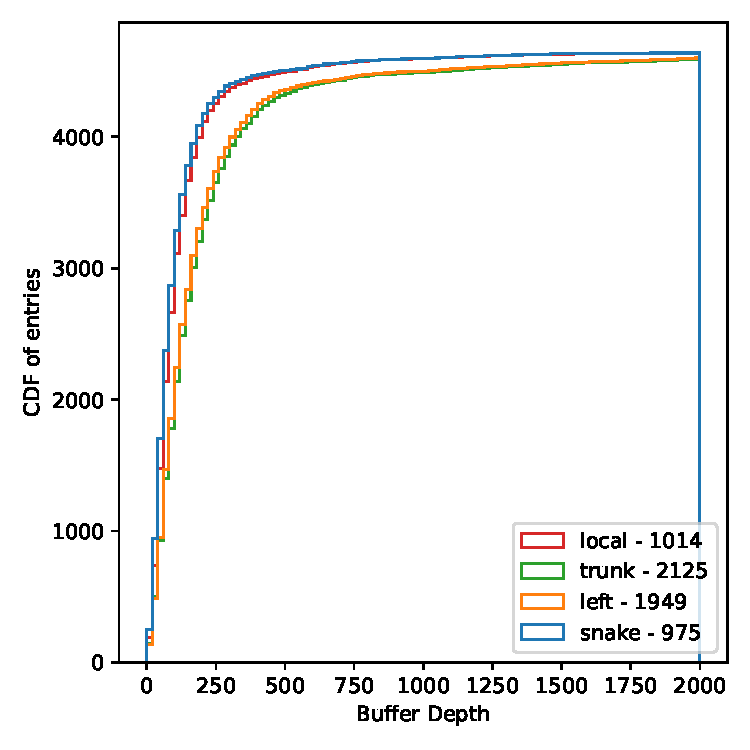
\includegraphics[width=\textwidth]{./images/mp60_16_slow_remote_stack.pdf}
      \caption[]%
      {{\small Routes Compared to Local}}    
  \end{subfigure}
  \vskip\baselineskip
  \begin{subfigure}[b]{0.475\textwidth}   
      \centering 
      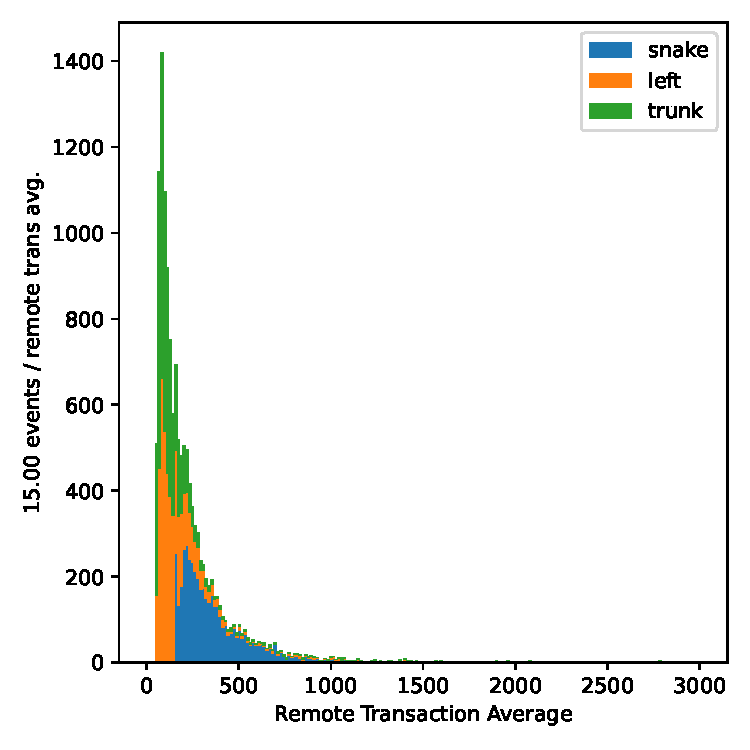
\includegraphics[width=\textwidth]{./images/mp60_16_slow_remote_transactions.pdf}
      \caption[]%
      {{\small Average Transactions}}    
  \end{subfigure}
  \hfill
  \begin{subfigure}[b]{0.475\textwidth}   
      \centering 
      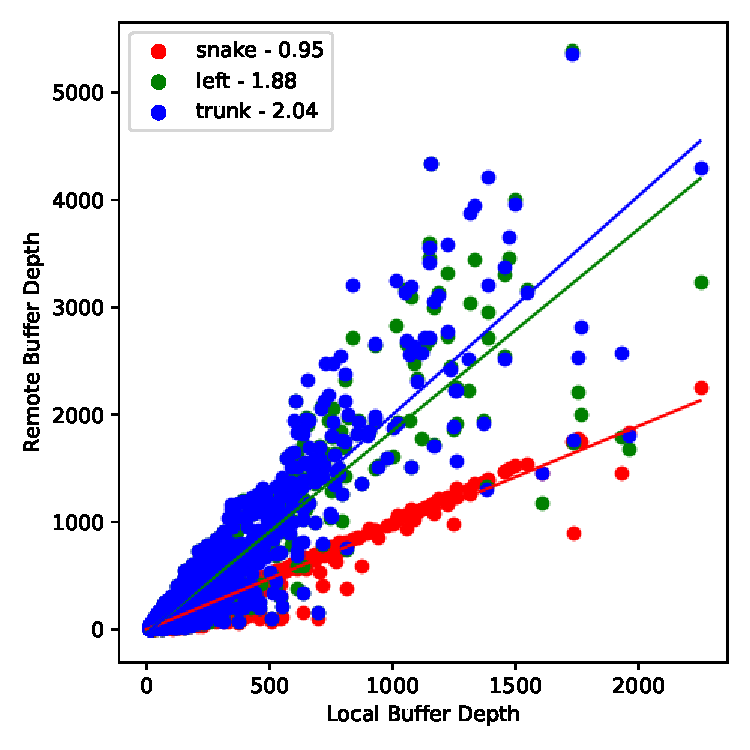
\includegraphics[width=\textwidth]{./images/mp60_16_slow_route_fits.pdf}
      \caption[]%
      {{\small Route Predictability}}    
  \end{subfigure}
  \caption[]
  {\small The results for a pull-based 4$\times$4 tile with 0.5\% frequency drift is shown. 
  Plot-(A) shows the cumulative integral of the number of events that are fully captured as a function of the local buffer depth.
  Plot-(B) includes the three tested routings against the local buffer depth. 
  The "Snake" routing is the only routing which limits the the remote FIFO depth near the local FIFO depth.
  Plot-(C) shows the relationship of the average number of transactions for all ASICs in each of the events.
  Plot-(D) is a scatter plot of the remote depth as a function of the local depth.
  The legend shows the slope values for linear best fits, which help guide the eye to show how the routes scale differently for large input events.
  } 
  \label{fig:mp60_slow_plots_for_digital_sim}
\end{figure*}

%%% Example of Digital Simulation Remote Parameterization
\begin{figure*}
  \centering
  \begin{subfigure}[b]{0.475\textwidth}
      \centering
      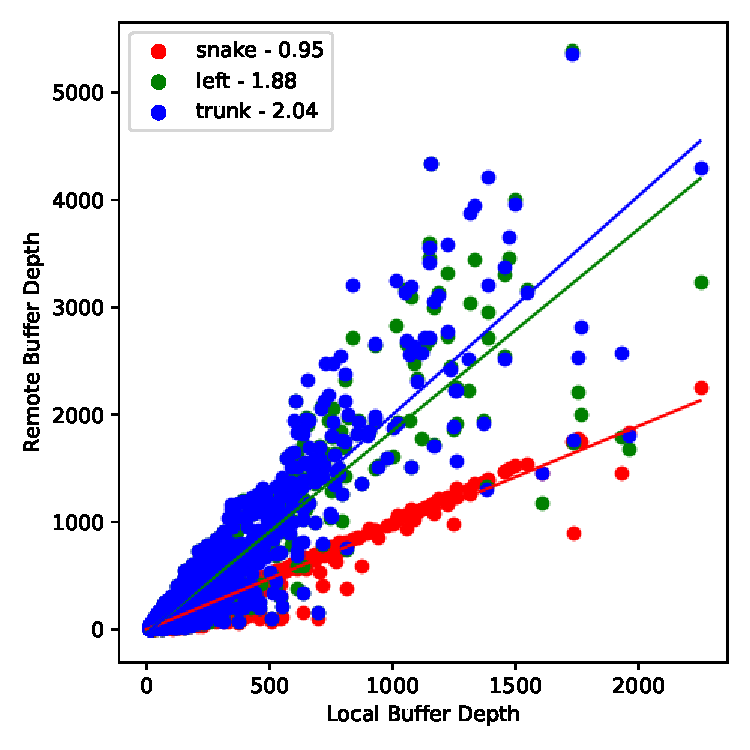
\includegraphics[width=\textwidth]{./images/mp60_16_slow_route_fits.pdf}
      \caption[]%
      {\small 4$\times$4 Tile}    
  \end{subfigure}
  \hfill
  \begin{subfigure}[b]{0.475\textwidth}  
      \centering 
      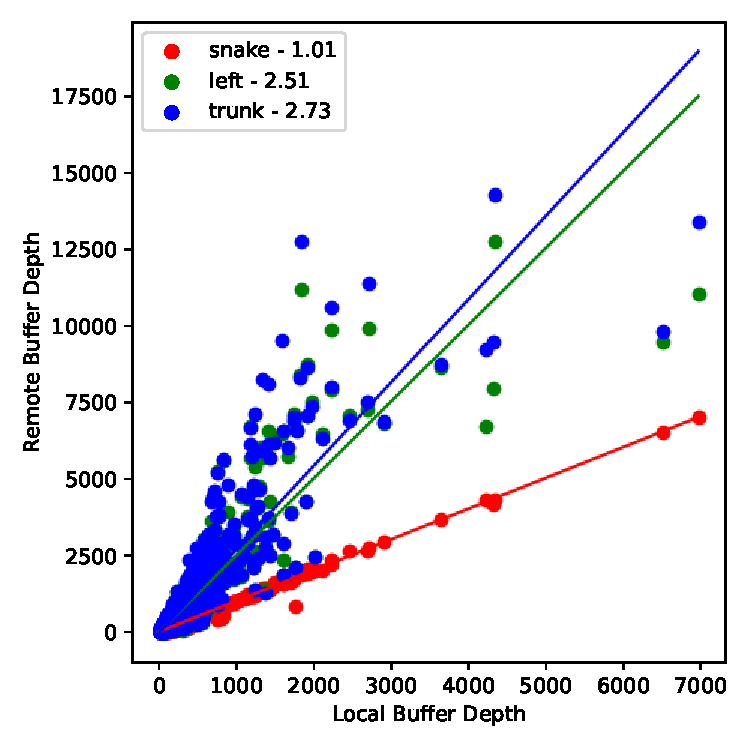
\includegraphics[width=\textwidth]{./images/mp60_64_slow_route_fits.pdf}
      \caption[]%
      {\small 8$\times$8 Tile}    
  \end{subfigure}
  \vskip\baselineskip
  \begin{subfigure}[b]{0.475\textwidth}   
      \centering 
      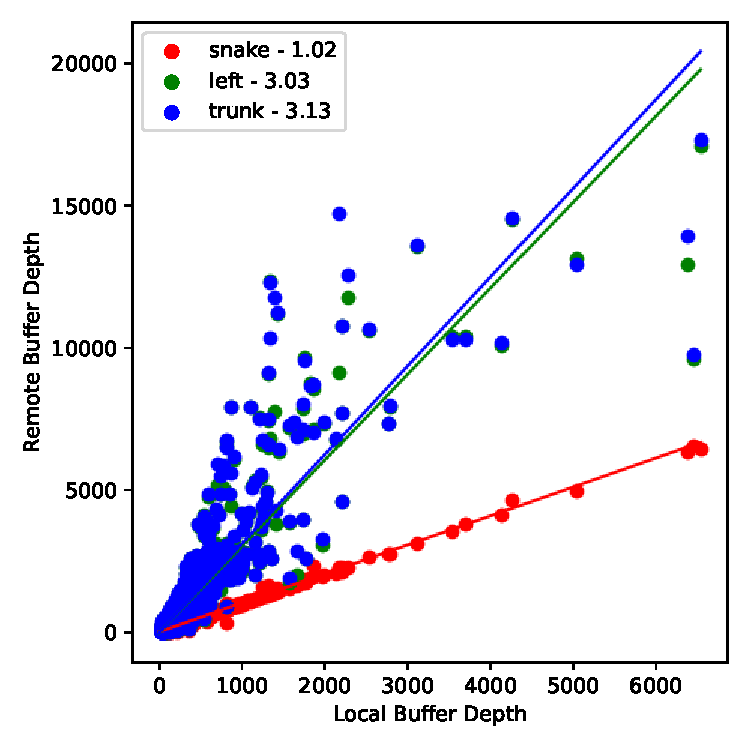
\includegraphics[width=\textwidth]{./images/mp60_140_slow_route_fits.pdf}
      \caption[]%
      {\small 10$\times$14 Tile}    
  \end{subfigure}
  \hfill
  \begin{subfigure}[b]{0.475\textwidth}   
      \centering 
      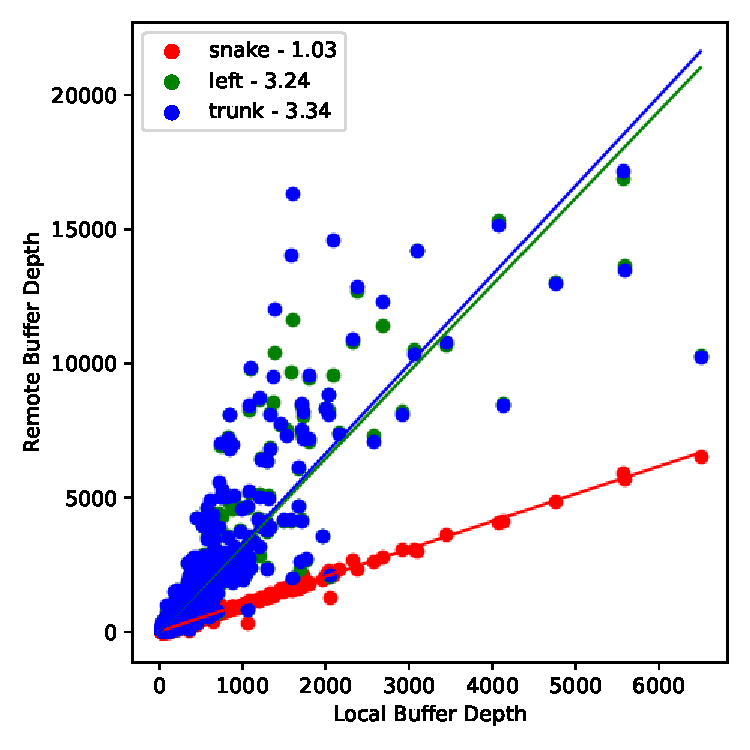
\includegraphics[width=\textwidth]{./images/mp60_256_slow_route_fits.pdf}
      \caption[]%
      {\small 16$\times$16 Tile}    
  \end{subfigure}
  \caption[]
  {\small A comparison of the remote vs local FIFO depths for different tile sizes is shown.
  Each plot corresponds to a different tile size with a frequency distribution of 0.5\%.
  Plot-(A) shows that even at small tile sizes (4$\times$4) the remote buffer depths do not predictability scale with the local depths
  Both the "Left" and "Trunk" routings slope's increase with the tile size to a maximum value over 3.
  Only the "Snake" routing maintains a predictable relationship between local and remote depths, as well as unit slope.
  These data indicate that any future routing for a Q-Pix tile, regardless of size, would need to dynamically route itself into a "Snake" routing in the event of SPF.
  } 
  \label{fig:compare_slow_plots_for_digital_sim_slow}
\end{figure*}

%%% Example of Digital Simulation Results for 16x16 tile
\begin{figure*}
  \centering
  \begin{subfigure}[b]{0.475\textwidth}
      \centering
      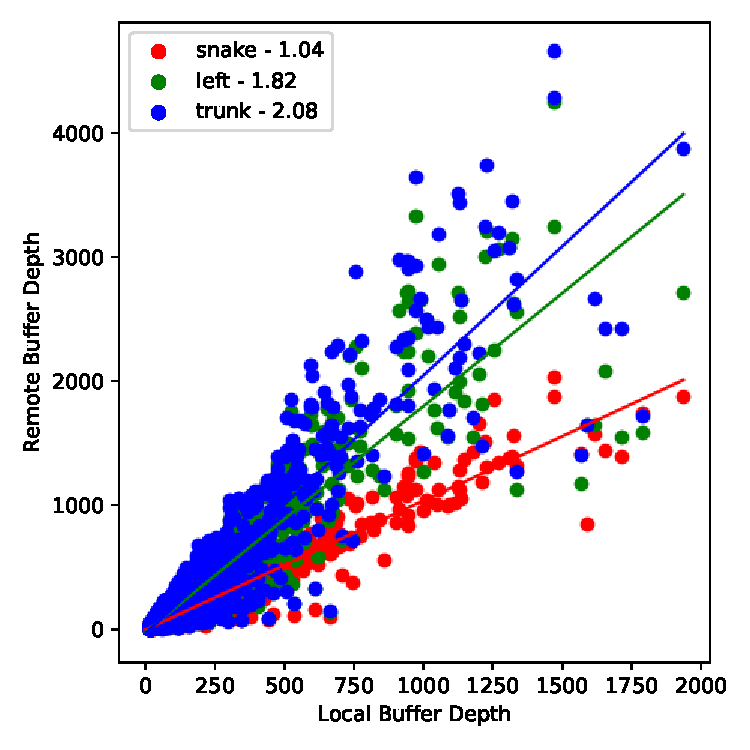
\includegraphics[width=\textwidth]{./images/mp60_16_fast_route_fits.pdf}
      \caption[]%
      {\small 4$\times$4 Tile}    
  \end{subfigure}
  \hfill
  \begin{subfigure}[b]{0.475\textwidth}  
      \centering 
      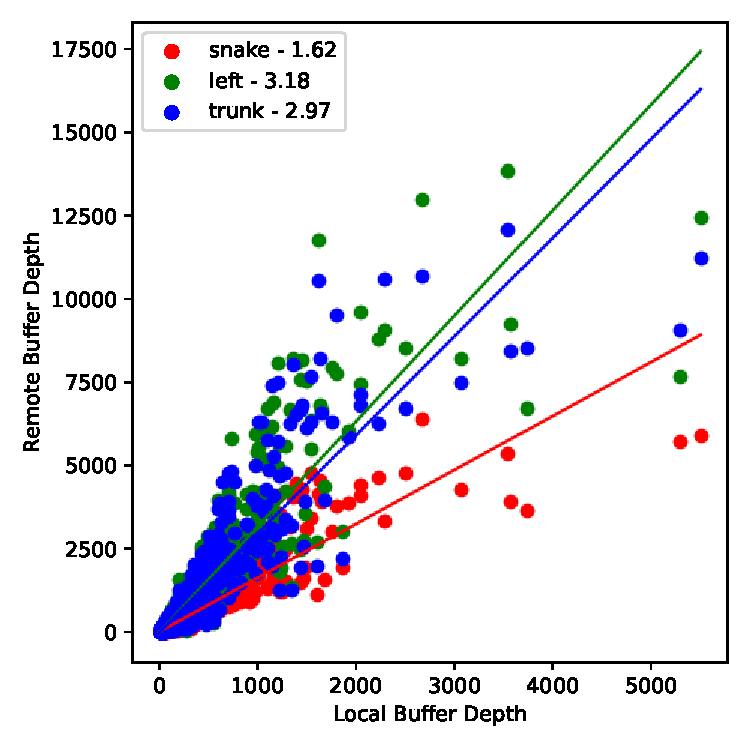
\includegraphics[width=\textwidth]{./images/mp60_64_fast_route_fits.pdf}
      \caption[]%
      {\small 8$\times$8 Tile}    
  \end{subfigure}
  \vskip\baselineskip
  \begin{subfigure}[b]{0.475\textwidth}   
      \centering 
      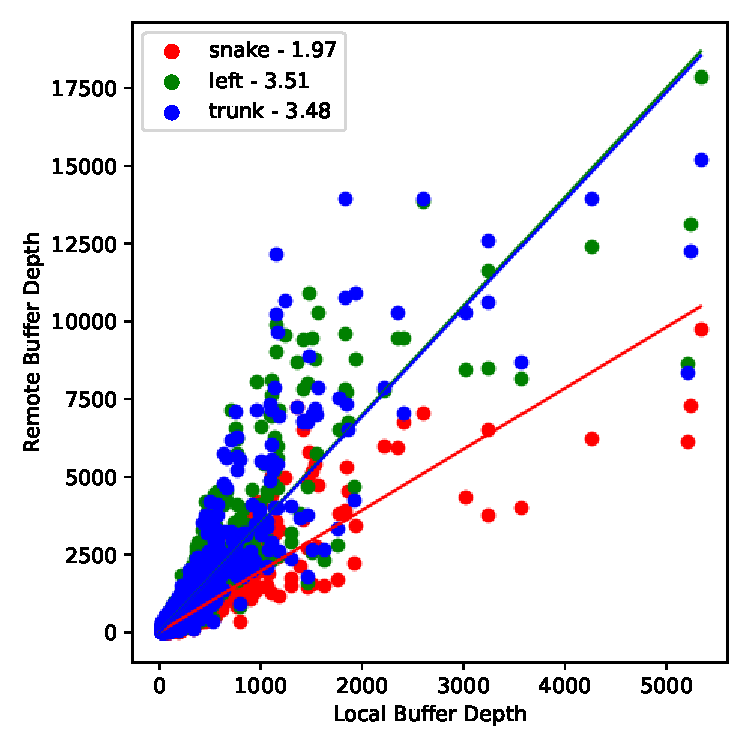
\includegraphics[width=\textwidth]{./images/mp60_140_fast_route_fits.pdf}
      \caption[]%
      {\small 10$\times$14 Tile}    
  \end{subfigure}
  \hfill
  \begin{subfigure}[b]{0.475\textwidth}   
      \centering 
      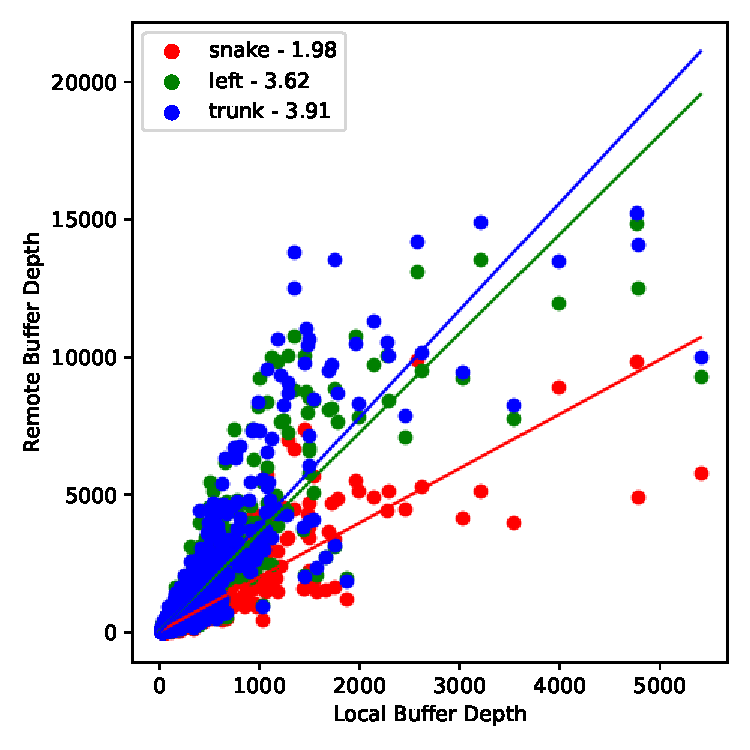
\includegraphics[width=\textwidth]{./images/mp60_256_fast_route_fits.pdf}
      \caption[]%v
      {\small 16$\times$16 Tile}    
  \end{subfigure}
  \caption[]
  {\small A comparison of the remote vs local FIFO depths for different tile sizes is shown.
  Each plot corresponds to a different tile size with a frequency distribution of 5\%.
  This plot is identical to Figure~\ref{fig:compare_slow_plots_for_digital_sim_slow}, except that the frequency distribution is 5\% instead of 0.5\%.
  These results indicate that low frequency variance between neighbor nodes is essential in order to have a predictable remote FIFO depth response based on the snake routing.
  Not only is the fit poor in Plot-(D) for the 16$\times$16 tile, but the slope has also doubled.
  This means that, on average, the requirement for the remote FIFO depth would be double that of the requirement on the local FIFO depth.
} 
  \label{fig:compare_fast_plots_for_digital_sim_fast}
\end{figure*}

%% table information
\begin{table}
	\begin{center}
		\begin{tabular}{|c|c|c|c|c|c|}
			\hline
			Freq. & Tile Size & Mean Local Hits & Snake & Left & Trunk \\
			\hline
			5\% & 16 & 48.250 & 423.293 & 166.403 & 138.380 \\
			\hline
			0.5\% & 16 & 51.846 & 449.861 & 177.357 & 147.346 \\
			\hline
			5\% & 64 & 34.129 & 1332.440 & 286.929 & 227.595 \\
			\hline
			0.5\% & 64 & 36.268 & 1400.794 & 301.775 & 239.087 \\
			\hline
			5\% & 140 & 26.521 & 2298.912 & 355.037 & 262.448 \\
			\hline
			0.5\% & 140 & 28.173 & 2416.778 & 373.173 & 275.614 \\
			\hline
			5\% & 256 & 24.343 & 4020.649 & 465.629 & 354.405 \\
			\hline
			0.5\% & 256 & 25.752 & 4209.196 & 487.090 & 370.695 \\
			\hline
		\end{tabular}
	\end{center}
	\caption{Transaction summary data is shown.
	The mean local hits column indicates the mean average of resets injected into the ASICs within the tile from an electron neutrino events.
	The Snake, Left, and Trunk, columns indicate the mean number of remote packet transactions which occured during the full 10 second simulation run.
	As expected, the amount of packet transactions in the snake routing scales with the tile size, whereas the Left and Trunk routings do not.
	The frequency distribution of the tiles does not affect the total number of transactions in the simulated event.
	These results can be used to indicate the amount of power and active time required for a tile to fully readout an electron neutrino event. 
	For example, if a tile size of 256 with a snake routing takes 4020 packets on average to digitize the event, then there are a total of slightly more than one million packets sent.
	If the amount of power used during single packet transaction is known, this ratio could be used to estimate the dissipated power during the back-end readout. 
	}
	\label{tab:transact}
\end{table}

%% table information
\begin{table}
	\begin{center}
		\begin{tabular}{|c|c|c|l|r|l|r|l|r|}
			\hline
			Freq. & Tile Size & Local Hits & 95-S & 99-S & 95-L & 99-L & 95-T & 99-T \\
			\hline
			5\% & 16 & 939 & 320 & 1014 & 535 & 1736 & 607 & 1971 \\
			\hline
			0.5\% & 16 & 1014 & 322 & 975 & 603 & 1949 & 652 & 2125 \\
			\hline
			5\% & 64 & 1200 & 598 & 2191 & 1098 & 4394 & 975 & 4295 \\
			\hline
			0.5\% & 64 & 1307 & 403 & 1328 & 970 & 4298 & 974 & 4521 \\
			\hline
			5\% & 140 & 1182 & 852 & 3486 & 1455 & 6558 & 1343 & 6309 \\
			\hline
			0.5\% & 140 & 1393 & 440 & 1464 & 1327 & 6616 & 1382 & 6757 \\
			\hline
			5\% & 256 & 1456 & 1039 & 3637 & 2026 & 7679 & 2008 & 8250 \\
			\hline
			0.5\% & 256 & 1670 & 527 & 1668 & 1773 & 7460 & 1784 & 7368 \\
			\hline
		\end{tabular}
	\end{center}
	\caption{Buffer Data}
	\label{tab:buffers}
\end{table}

%% table information
\begin{table}
	\begin{center}
		\begin{tabular}{|c c|c|c|c|c|}
			\hline
			Tile Size & Frequency & Snake & Left & Trunk & Push \\
			\hline
			16 & 0.5\% & 0.948 & 1.879 & 2.039 & 0.979 \\
			& 5\% & 1.041 & 1.823 & 2.082 & 1.031 \\
			\hline
			64 & 0.5\% & 1.006 & 2.514 & 2.727 & 0.999 \\
			& 5\% & 1.623 & 3.176 & 2.969 & 1.11 \\
			\hline
			140 & 0.5\% & 1.021 & 3.033 & 3.131 & na \\
			& 5\% & 1.966 & 3.506 & 3.481 & na \\
			\hline
			256 & 0.5\% & 1.027 & 3.243 & 3.336 & na \\
			& 5\% & 1.981 & 3.616 & 3.913 & na \\
			\hline
		\end{tabular}
	\end{center}
	\caption{Transaction fit summary results.
	The values shown from the fits indicate the linear fit to the results to predict the relationship between the local and remote FIFO depth requirements.
	Push fit data is not available for larger tiles (140 and 256) due to simulation time constraints.
	}
	\label{tab:fit}
\end{table}

\section{Summary and Further Studies}~\label{sec:further_studies}

The results presented in this section provide first physical analysis of the Q-Pix digital readout.
Included in the analysis are long exposure to radiogenic background sources, leakage current, neutrino beam events, and the response of the digital back-end ASICs.
All events occur in a 2.3$\times$6.0~\unit{m^{2}} LAr container, with a maximum drift distance of 3.6~\unit{m}.
The parameters of the Geant4 simulation are identical to those in Table two from~\citep{qpix:shion} with the exception that the sampling time is configured to each digital node as described in Section~\ref{sec:hits}.
The flux of beam neutrino events are taken from~\ref{dune_2021_near_detector_cdr} also using GENIE~\citep{Andreopoulos:2009rq} v2.12.10.

We find that the digital back-end readout permits the ability to fully capture 99\% events from beam neutrino events up to 10~\unit{GeV} provided the local FIFO depth is at least 426.
Each ASIC would be able to record all resets from these neutrino events regardless of incident neutrino momentum direction if the local FIFO depth is 1670.
These results present an expected upper-bound of the required local and remote FIFO depths for the digital ASIC, since most electrons of reconstructed energy for neutrino oscillations (See Chapter 5 from~\citep{DUNE_TDRv3_Abi_2020}) expected to be less than 4~\unit{GeV}, while the analysis presented here are for events up to 10~\unit{GeV}.

The current Q-Pix digital prototype allows for dynamic and configurable routing. 
We find that the only stable relationship between the local FIFO depth and the remote FIFO depth occurs for the "Snake" based routing, where the required depths are approximately equal.
Additionally, the relationship between these FIFO depths are independent of tile size, which imply that tiles of any size should reconfigure itself to always have an effective "Snake" routing in the event of SPF.

We also find no difference in the ability of a "push" architecture to better alleviate neutrino events than the current "pull" based architecture.
The reason for this is due to the quick arrival time of neutrino resets compared to the average packet transaction time.

In order for a "push" architecture to be able to reduce both the remote and local FIFO depth requirements the average packet transaction time would have to be small compared to the average RTD on each node. 
The total decrease of the packet transaction time will likely have to be an order of magnitude, or more, according to Figure~\ref{fig:example_rtd_scatter}
The distribution of RTDs for the example scatter event clearly indicate that most of the resets come within 1~\unit{\mu s} of each other.
Since the current packet transaction time is, on average $\approx 50~\unit{\mu s}$, for the push architecture to transfer packets more quickly than they arrive the packet transaction time would have to decrease by about a factor of 50.

A combination of changes could make this possible: a faster local oscillator, a different communication protocol, and zero-suppresion on some packet data.
Future designers will have to ask themselves if a redesign of the digital clock, the packet communication protocol, and/or the FSM of the digital ASIC is easier than increasing two FIFO depths.
It is the humble opinion of the author of this work that it is not.

\begin{figure}[]
\centering
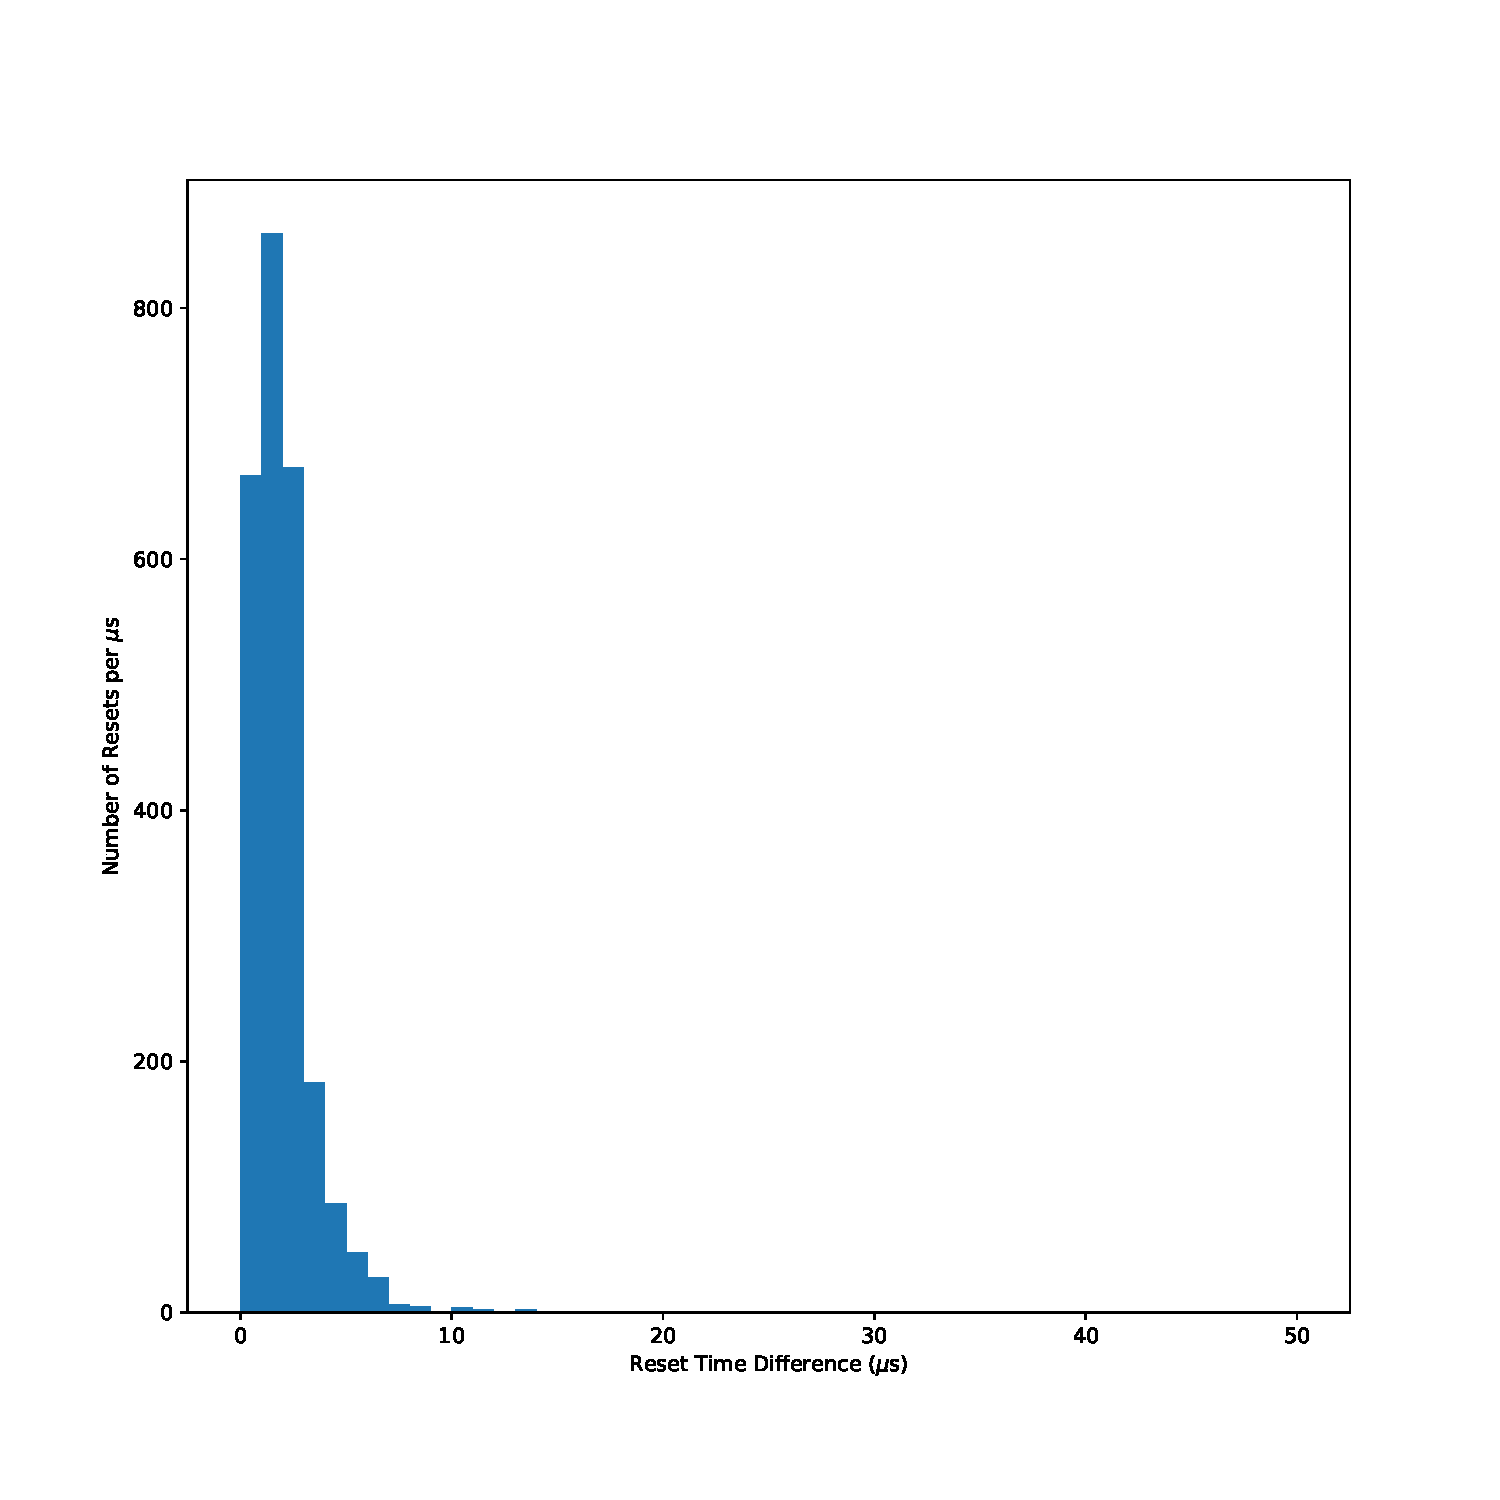
\includegraphics[width=0.7\textwidth]{images/example_rtd_scatter.pdf}
\caption{A caluclation of all of the Reset Time Differences (RTDs) for the example scatter event shown in Figure~\ref{fig:compare_integral}.
A packet transaction takes $\approx$ 50~\unit{\mu s} to occur.
The distribution of RTDs for a scatter event indicate that most of the resets occur separated by less than 1~\unit{\mu s}.
}
\end{figure}~\label{fig:example_rtd_scatter}

Finally, we remark how much the digital ASIC is capable of, despite it's seemingly simple design~\ref{sec:digital_fsm}.
In the spirit of the Q-Pix's principle of least action, we assert that the digital ASIC should be also be as simple as possible while relaying all data required for the application.
